%% tex/NPClass.tex
%% Copyright 2019 Andrea Berlingieri
%
% This work may be distributed and/or modified under the
% conditions of the LaTeX Project Public License, either version 1.3
% of this license or (at your option) any later version.
% The latest version of this license is in
%   http://www.latex-project.org/lppl.txt
% and version 1.3 or later is part of all distributions of LaTeX
% version 2005/12/01 or later.
%
% This work has the LPPL maintenance status `maintained'.
%
% The Current Maintainer of this work is Andrea Berlingieri.
%
% This work consists of all files listed in manifest.txt
\chapter{La classe $\NPClass$}

%Slide 105
Vediamo ora due argomenti importanti concentrando la nostra attenzione su una classe di complessità
molto interessante: $\NPClass$. I due argomenti che trattiamo sono il teorema della proiezione e la
nozione di riducibilità.

\section{Teorema della proiezione}

Il teorema della proiezione è importante perché mette in relazione le due visioni della classe
$\NPClass$: una, che la definisce, è quella di insieme dei linguaggi riconoscibili da una macchina
non deterministica, e l'altra, interessante a livello pratico, è quella di insieme dei problemi per
cui esistono algoritmi di verifica della soluzione che operano in tempo polinomiale.

\begin{thm}
    \textbf{(Teorema della proiezione).} Dato un linguaggio $A \subseteq \Sigma^{*}$, $A \in
    \NPClass$ se e solo se esiste un linguaggio $B \in \PClass$ e un polinomio $p$ tale che per ogni
    $x \in \Sigma^{*}$
    \begin{equation*}
        x \in A \iff \exists y, |y| \leq p(|x|) \land \pair{x}{y} \in B
    \end{equation*}
\end{thm}

$y$ è un certificato che dipende da $x$. È un'informazione aggiuntiva rispetto ad $x$ che ci
permette di fare una verifica veloce. È una sorta di ``prova'' che $x$ appartiene in effetti al
linguaggio $A$. L'utilità di $B$ sta nel fatto che ci permette di verificare in tempo polinomiale
l'autenticità del certificato per $x$.

Che cosa sia il cerficicato non è ben definito: dipende dal problema e sta a noi definire cosa sia
un buon cerificato. Dato che noi consideriamo solo problemi decisionali il certificato può essere
qualunque informazione che ci permetta di verificare che la risposta sia ``Sì''.

Chiediamo inoltre che la dimensione del certificato non cresca esponenzialmente. Il motivo è che
input grandi ci danno complessità basse che sono tuttavia fittizie, un pò come accadeva per il
padding.

Ad esempio per il problema della tautologia abbiamo un algoritmo lineare nella dimensione di una
tabella di verità che verifica se la tabella è ben formata, e quindi se una formula data è
tautologica. Tuttavia questa tabella ha dimensione esponenziale. L'algoritmo risulta efficiente se
confrontato con la dimensione della tabella, ma risulta pessimo se confrontato con la dimensione del
nostro input, ovvero la formula di partenza. Di conseguenza non si tratta di un buon certificato per
noi.

\begin{proof}

    Sia $A \subseteq \Sigma^{*}$, $A \in \NPClass$ e sia $x$ una stringa in $A$. Abbiamo che $A \in
    \NPClass$ sse esiste una MdTN $M$ che riconosce $A$. Che certificato possiamo dare per $x$?
    Come certificato possiamo prendere la sequenza delle scelte prese da $M$ in una computazione che
    riconosce $x$, insieme a $\code{M}$. Quanto è grande questa sequenza? È polinomiale in $|x|$,
    essendo $A \in \NPClass$. Esiste quindi un cammino accettante polinomiale nel numero di passi.
    Il codice di $M$ è costante nella sua dimensione e non influisce a livello della complessità.
    Sia $B$ il linguaggio delle coppie $x$-certificato. Dato $x$ ed il suo certificato una macchina
    deterministica $M'$ che riconosce il linguaggio $B$ effettua una simulazione di $M$ usando le scelte
    fornite. Se la configurazione finale della simulazione di $M$ è accettante la machina $M'$
    accetta la coppia $x$-certificato; in caso contrario rifiuta. È facile verificare il secondo $\iff$
    dell'enunciato del teorema data questa definizione di $M'$ e $B$. Inoltre abbiamo che $B \in
    \PClass$, dato che l'estrazione del certificato dalla coppia è un'operazione con complessità
    lineare rispetto alla dimensione di questa e la simulazione di $M$ richiede un numero di passi
    polinomiale in $|x|$.

    Viceversa supponiamo ora di avere $B \in \PClass$. Vogliamo dimostrare che se prendiamo un
    polinomio $p$ e facciamo la proiezione esistenziale bound da $p$ abbiamo che il linguaggio
    ottenuto in questo modo sta in $\NPClass$. In particolare vogliamo dimostrare che il linguaggio
    \begin{equation*}
        A = \set{x \mid \exists y, y \leq p(|x|) \land \pair{x}{y} \in B}
    \end{equation*}
    fa parte di $\NPClass$.

    Per mostrare ciò esibiamo una MdTN $M$ che ci permetta di riconoscere $A$. $M$ funziona nel
    seguente modo: dato $x$ genera tutti i certificati $y$ di dimensione minore o uguale a $p(|x|)$
    e testa l'appartenenza di $\pair{x}{y}$ a $B$ in tempo polinomiale per tutti. Se uno di questi
    certificati risulta valido $M$ accetta $x$, altrimenti rifiuta. La quantità di certificati da
    testare è esponenziale, dato che il numero di certificati diversi di lunghezza $p(|x|)$ è
    $|\Sigma|^{p(|x|)}$. Sfruttando il fatto che la macchina deterministica è ``fortunata''
    generiamo non deterministicamente il certificato corretto per $x$. $M$ riconosce quindi $x
    \in A$ in tempo polinomiale non deterministico.

\end{proof}

Non è restrittivo supporre, come abbiamo fatto implicitamente, che $B$ sia un linguaggio sullo
stesso alfabeto $\Sigma$ di $A$.

\section{Riducibilità}

%Slide 112

La nozione di riducibilità che vediamo è molto simile a quella della teoria della complessità.

\begin{defn}
    Siano $A,B \in \Sigma^{*}$ due linguaggi. Diremo che $A$ è riducibile in tempo polinomiale a
    $B$, $A \leq_{p} B$, se esiste $f \in \FP$ tale che per ogni $x \in \Sigma^{*}$, $x \in A \iff
    f(x) \in B$.
\end{defn}
Se al vincolo polinomiale alla complessità di $f$ andiamo a sostituire un diverso vincolo sulla
complessità in tempo o in spazio otteniamo una nozione di riducibilità analoga a questa ma diversa
nel numero e nella natura delle riduzioni.

La nozione di riducibilità è many-to-one. Vogliamo che $f$ sia calcolabile in tempo polinomiale.
Nella definizione di riducibilità dobbiamo fare attenzione ad un dettaglio tecnico.  Dire che $f
\in \PClass$ è sbagliato perché $f$ non è un linguaggio, bensì una funzione. Per questo motivo
introduciamo $\FP$ come l'insieme delle funzioni calcolabili in tempo polinomiale, ovvero delle $f$
per le quali esiste una MdT che calcola $f$ in tempo polinomiale.

Qualunque tipo di nozione di riducibilità è ragionevole. Più sono deboli i vincoli che poniamo
alla complessità di $f$ più la nostra nozione di riduzione sarà lasca e maggiori saranno le
riduzioni possibili. Intuitivamente se disponiamo di un numero elevato di risorse è più facile
ridurre un linguaggio ad un altro, mentre se le risorse disponibili sono limitate le riduzioni
possibili diminuiscono. Ad esempio una riducibilità esponenziale permetterebbe di ridurre molti
problemi tra loro. Noi ci concentriamo unicamente sulla riducibilità polinomiale in tempo. È
generalmente la più interessante.

Le riducibilità sono in genere dei preordini. Ricordiamo che un preordine è una relazione binaria
riflessiva e transitiva. Per la riducibilità polinomiale in tempo la proprietà riflessiva è
dimostrabile in maniera ovvia. Per la transitività supponiamo di avere $A,B,C$ con $A \leq_{p} B$
attraverso $f$ e $B \leq_{p} C$ attraverso $g$. Ci basta comporre $f$ e $g$ per ottenere $h$
calcolabile con complessità polinomiale che riduce $A$ a $C$. Questa composizione ha complessità
polinomiale perché la composizione di polinomi è ancora un polinomio. Questo vale anche per
$\leq_{L}$, la riducibilità in $\LOGSPACE$.

%Slide 113

\begin{defn}
    Sia $\CClass$ una classe di linguaggi e sia $\leq$ un qualche preordine. Diremo che $\CClass$ è
    chiusa rispetto a $\leq$ se
    \begin{equation*}
        A \leq B \land B \in \CClass \implies A \in \CClass
    \end{equation*}
\end{defn}

Si può dimostrare che che $\PClass$, $\NPClass$ e $\PSPACE$ sono chiuse rispetto alla riduzione
polinomiale.

Supponiamo infatti di avere due linguaggi $A$ e $B$, con $B \in \PClass$, e di voler riconoscere il
linguaggio $A$. Sia $x$ la stringa che vogliamo riconoscere. Se esiste una funzione di riduzione $f
\in \FP$ da $A$ a $B$ possiamo calcolare la riduzione $f(x)$ in tempo polinomiale.  Sappiamo che la
dimensione di $f(x)$ sarà polinomiale rispetto alla dimensione di $x$, dato che $f$ è stata
calcolata in tempo polinomiale e lo spazio è bound dal tempo. Inoltre verificare che $f(x) \in B$
richiede tempo polinomiale. Poichè la composizione di polinomi rimane un polinomio questa procedura
di riconoscimento di $A$ ha complessità polinomiale. Lo stesso discorso si applica se al posto di
$\PClass$ abbiamo $\NPClass$.

Una classe come $\LOGSPACE$ non è chiusa rispetto alla riducibilità in tempo polinomiale. È chiusa
rispetto alla riducbilità in spazio logaritmico. Supponiamo che $B \in \LOGSPACE$ e che $A \leq_{p}
B$. Questo non implica che $A \in \LOGSPACE$. Già il valore di $f(x)$ può avere dimensione
polinomiale, e lo spazio logaritmico non ci basta. Il problema è che questa nozione di riducibilità
è troppo lasca per la classe che che stiamo considerando, ovvero $\LOGSPACE$. Di conseguenza ce ne
servirebbe una più precisa.

La classe $\PClass$ non è chiusa rispetto alla riduzione esponenziale. Infatti possiamo ridurre un
qualsiasi problema $A$ in tempo esponenziale ad uno più semplice $B \in \PClass$. Questo non
implica che abbiamo un algoritmo per risolvere $A$ in tempo polinomiale e che quindi $A \in
\PClass$.

Vedremo che tutti i problemi non banali in $\PClass$ sono mutuamente riducibili con una riduzione
polinomiale. Inoltre tutti i problemi in $\EXP$ sono $\EXP$-completi. Infine esiste una riduzione
esponenziale da un problema in $\EXP$ ad uno in $\PClass$.

%Slide 114

\section{$\NPClass$-completezza e $\NPClass$-hardness}

La definizione di problema arduo e problema completo può essere data per qualsiasi classe di
complessità. Noi siamo interessati a $\NPClass$.

\begin{defn}
    Sia $\CClass$ una classe di linguaggi e $\leq$ un preordine tra di essi. Sia $B$ un linguaggio.
    Abbiamo che
    \begin{itemize}
        \item $B$ e $\CClass$-arduo rispetto a $\leq$ se ogni $A \in \CClass$ è riducibile a $B$;
        \item $B$ e $\CClass$-completo rispetto a $\leq$ se $B \in \CClass$ e $B$ è $\CClass$-arduo;
    \end{itemize}
\end{defn}

Un problema $\CClass$-arduo è il problema più complicato della classe. Questa nozione di
complicatezza però dipende dalla quantità di risorse che diamo alla nozione di riducibilita.  Meno
risorse diamo alla funzione di riduzione, meno sono le riduzioni possibili, e più fini sono le
distinzioni tra classi, e analogamente con più risorse vale il contrario.

\begin{defn}
    Sia $B$ un linguaggio. Diciamo che $B$ è $\NPClass$-hard se $\forall A \in \NPClass, A \leq_{p}
    B$. Diciamo che $B$ è $\NPClass$-completo se $B$ è $\NPClass$-hard e inoltre $B \in \NPClass$.
\end{defn}

I problemi $\NPClass$-completi sono quei problemi a cui tutti gli altri sono riducibili. Se avessimo
un modo efficiente per risolvere un problema $\NPClass$-completo $A$ sapremmo che, per ogni altro
problema in $\NPClass$, esisterebbe un algoritmo efficiente di soluzione che utilizza una riduzione
polinomiale dal problema da risolvere ad $A$ e l'algoritmo per $A$.

L'$\NPClass$-completezza è interessante a livello pratico. Un problema che sappiamo essere
$\NPClass$-completo è $\SAT$. Esistono algoritmi molto efficienti che possono risolvere $\SAT$
nonostante la loro complessità nel caso pessimo rimanga esponenziale. Si utilizzano proprietà di
sottoclassi particolari di formule proposizionali che permettono di avere algoritmi di soluzione
generalmente efficienti. Non è una cattiva idea risolvere un problema trovando una riduzione
polinomiale a $\SAT$ e usare un $\SAT$-solver, dato che $\SAT$ è stato molto investigato ed esistono
algoritmi ed euristiche efficienti. Si potrebbe fare la stessa cosa utilizzando altri problemi
$\NPClass$-completi.

Non si sa se tutti i problemi in $\NPClass$ sono $\NPClass$-completi. Per $\PClass$ questa cosa
invece vale.  Se riusciamo a dimostrare che esiste un problema in $\NPClass$ non $\NPClass$-completo
abbiamo come conseguenza che
$\PClass \not= \NPClass$.

%Uguaglianza di Leibniz: $x = y \iff \forall P, P(x) \iff P(y)$. Due oggetti sono uguali se qualsiasi
%osservazione facciamo su di essi otteniamo lo stesso risultato. Se dimostriamo che c'è qualche
%proprietà che vale per un $x$ ma non per un $y$ abbiamo che $x \not= y$.

La questione $\PClass$ vs $\NPClass$, ovvero determinare se queste due classi coincidono o sono
diverse, è uno dei Millenium Problems. C'è in palio un premio di 1 milione di dollari per chi
fosse in grado di risolvere questo problema, o fare comunque passi importanti verso la risoluzione.
Si congettura che $\PClass \not= \NPClass$.

Una problematica ancora aperta e altrettanto interessante è la dimostrazione che l'inclusione tra
$\PClass$ e $\PSPACE$ è stretta. $\PSPACE$ è una classe molto grande, che contiene anche
$\NPClass$, e molto distante da $\PClass$. Si congettura che l'inclusione sia stretta, ma non si è
ancora riusciti a dimostrarlo. Un problema con questa dimostrazione è legato al fatto che le due
classi sono definite da risorse diverse. Lavorare con risorse diverse a livello di complessità è
sempre delicato e non banale.

%Slide 116

\subsection{Problemi $\NPClass$-completi}

Vediamo un esempio di problema $\NPClass$-completo

Dimostrare la completezza di un problema non è ovvio. Infatti dobbiamo dimostrare che tutti i
problemi in $\NPClass$ sono riducibili al problema che vogliamo dimostrare essere completo.

Il problema che consideriamo è il problema limitato della fermata con macchine non deterministiche.

\begin{thm}
    Sia $\BHP$ il linguaggio così definito:
    \begin{equation*}
        \BHP = \set {\tuple{x,y,0^{t}} \mid \text{La MdTN $M$ accetta $y$ in tempo
        $\textit{time}_{M_{x}}(y) \leq t$}}
    \end{equation*}
    $\BHP$ è $\NPClass$-completo
\end{thm}

Il tempo è dato in formato unario. Di solito si fa così quando vogliamo una complessità lineare
in un dato tempo.  Se dessimo una rappresentazione logaritmica del tempo l'algoritmo che lavora con
quel tempo risulterebbe avere complessità esponenziale.

\begin{proof}
    La prima cosa da fare è dimostrare che questo problema sta in $\NPClass$. Costruiamo una MdTN
    $M$ che riconosce $\BHP$. $M$ opera nel seguente modo: verifica innanzitutto che la stringa in
    input sia una tripla la cui prima componente sia il codice di una MdTN. Dopodiché simula la
    computazione della macchina $M_{x}$ su input $y$ con bound dato da $t$. Ad ogni scelta non
    deterministica di $M_{x}$ corrisponde una scelta non deterministica di $M$. Se alla fine della
    simulazione abbiamo che $M_{x}$ riconosce $y$ abbiamo che $M$ accetta, altrimenti rifiuta.
    Rifiuta inoltre se la simulazione supera il bound in tempo.

    Supponiamo ora di avere un linguaggio $A \in \NPClass$ e di volerlo riconoscere, ovvero decidere
    $y \in A$.  Possiamo farlo con una riduzione polinomiale a $\BHP$: prendiamo il codice $x$ di
    una MdTN $M$ che riconosce $A$ in tempo polinomiale, l'input $y$ da riconoscere e come tempo $t$
    prendiamo $p(|y|)$, dove $p$ è il polinomio che fa da bound alla complessità di $M$. Abbiamo
    che $y \in A \iff \tuple{x,y,0^{t}} \in \BHP$.
\end{proof}

$\BHP$ non è stato molto investigato. Dal punto di vista pratico non è il miglior problema a cui
ridursi. La costruzione di $\BHP$ inoltre è un pò artificiosa, serve giusto a dimostare che
esistono problemi $\NPClass$-completi.

Si poteva dimostrare inoltre che $\BHP \in \NPClass$ mostrando un certificato per esso ed un
algoritmo efficiente di verifica. In questo caso un certicato poteva essere la sequenza delle
decisioni prese dalla macchina $M_{x}$ su input $y$ e la verifica sarebbe consistita nella
simulazione di $M_{x}$ su input $y$ seguendo la sequenza di istruzioni data dal certificato.

%Slide 116

%Un problema NP-completo è un problema jolly, tale che ogni problema in NP può essere ridotto ad
%esso.
\section{$\textsc{sat}$ è $\NPClass$-completo}

Abbiamo visto che esiste un problema $\NPClass$-completo: $\BHP$. Ne vediamo ora uno più importante
a livello pragmatico.

%Slide 119

Il problema $\NPClass$-completo a cui siamo interessati è $\SAT$. È stato il primo problema ad
essere stato dimostrato essere $\NPClass$-completo. È un problema reale, di rilevanza pratica, ed
ha senso chiedersi quale sia la sua complessità.

$\SAT$ è il problema della soddisfacibilità delle formule della logica proposizionale. Data una
formula della logica proposizionale ci chiediamo se esiste un assegnamento di valori di verità alle
variabili proposizionali che soddisfi la formula.
\begin{equation*}
    \SAT = \set{\varphi \mid \text{$\varphi$ è soddisfacibile}}
\end{equation*}

La dimostrazione della completezza di $\SAT$ è complessa a livello formale, come tutte le
dimostrazioni dirette della $\NPClass$-completezza di un problema.

È ovviamente in $\NPClass$, dato che abbiamo un algoritmo polinomiale per verificare la correttezza
di una soluzione: se come certificato prendiamo l'assegnamento di valori alle variabili
proposizionali la verifica che questo assegnamento renda la formula vera può essere fatto in tempo
lineare nella dimensione della formula. È complicato invece dimostrare che è $\NPClass$-completo,
poichè è complicato dimostrare che $\SAT$ è $\NPClass$-arduo. Dobbiamo dimostrare che, dato un
qualsiasi problema  $A \in \NPClass$, abbiamo che $A \leq_{p} \SAT$. Non possiamo fare ipotesi
ulteriori su $A$ oltre l'appartenenza a $\NPClass$.

In generale abbiamo due modi per dimostrare che un problema $A$ è $\NPClass$-arduo.
%Questa è di solito la parte difficile nel dimostrare che $A$ è completo.
Un modo è quello diretto, che utilizza la definizione di $\NPClass$-hardness. L'altro modo è, se
abbiamo un $B$ $\NPClass$-arduo, ridurre $B$ ad $A$:
\begin{equation*}
    B\text{ è $\NPClass$-arduo} \land B \leq_{p} A \implies \text{$A$ è arduo}
\end{equation*}
Quest'ultimo è il modo più semplice e deriva dalla transitività della nozione di riducibilità.

Potremmo quindi dimostrare l'arduità di $\SAT$ riducendo, ad esempio, $\BHP$ a $\SAT$. Questa è la
tecnica più comunemente usata, in genere con riduzioni da $\SAT$ o $3\SAT$ al nostro problema di
interesse.

Per dimostrare che un problema $A$ è $\NPClass$-arduo è tipicamente conveniente scegliere uno dei
tanti problemi $\NPClass$-ardui che assomiglia ad $A$ e ridurlo a quest'ultimo. La possibilità di
scegliere il problema ci dà molta flessibilità, e rende più semplici le riduzioni. Spesso le
riduzioni non sono ovvie, richiedono un certo lavoro creativo.

Se non avessimo problemi $\NPClass$-completi l'unica via per dimostrare che $\SAT$ è arduo sarebbe
quella diretta. Questa era la situazione quando venne dimostrata per la prima volta la
$\NPClass$-completezza di $\SAT$. Noi condurremo la dimostrazione come se questo fosse il caso.

\begin{thm}
    \textbf{(Teorema di Cook-Levin).} $\SAT$ è $\NPClass$-completo
\end{thm}
\begin{proof}

    Sappiamo già che $\SAT \in \NPClass$. Sia $A \in \NPClass$. Dobbiamo mostrare una riduzione da
    $A$ a $\SAT$, ovvero una funzione $\varphi$ in $\FP$ tale che $\forall x. x \in A \iff
    \varphi_{x} \in \SAT$, dove $\varphi_{x}$ si ottiene da $\varphi$ e $x$. $\varphi_{x}$ è una
    formula proposizionale, che vogliamo sia soddisfacibile se $x \in A$ e insoddisfacibile
    altrimenti.

    Cosa sappiamo di $A$? Che $A \in NP$. Perciò esiste una MdTN $M$ che lavora in tempo
    polinomiale tale che $A = \Lang_{M}$.

    Abbiamo che $\varphi_{x}$ dipende anche da $M$ e dal polinomio che fa da bound al tempo di
    riconoscimento di $M$. Avremo quindi una $\varphi_{x}^{M,p}$.

    L'intuizione è che $x \in A$ se esiste una computazione non deterministica bound da $p$ che
    porta ad una configurazione di accettazione. Vogliamo quindi una formula che esprima questa
    condizione e che sia soddisfacibile se esiste una computazione che porta ad accettazione di $x$
    in tempo $p$ e insoddisfacibile altrimenti.

    Se avessimo un linguaggio più espressivo, ad esempio del prim'ordine, sarebbe più semplice
    esprimere questa condizione. Infatti un linguaggio del prim'ordine è abbastanza espressivo da
    esprimere la semantica di una macchina di Turing. A questo punto sarebbe facile costruire una
    formula del prim'ordine che sia soddisfacibile se esiste una computazione accettante per $x$.
    Questo dimostra, implicitamente, che il problema della soddisfacibilità, o anche quello della
    verità, in logica del prim'ordine è un problema arduo. Questo non sorprende, dato che la
    logica del prim'ordine è complicata e indecidibile. Qui abbiamo però la logica proposizionale,
    che non è altrettanto espressiva.  Dobbiamo trovare un modo per esprimere questa esistenza
    della computazione accettante.

    La nostra formula deve esprimere l'esistenza di una computazione di $M$ su $x$ di durata
    $p(|x|)$. Come possiamo descrivere questa computazione? Ad esempio con una matrice, in cui ogni
    riga della matrice sarà una descrizione del nastro della macchina in un determinato istante.
    Possiamo supporre che $M$ abbia un solo seminastro. Questo non limita il potere espressivo.

    Quante descrizioni, ovvero righe, ci servono? $p(|x|)$, dato che il numero di righe corrisponde
    al numero delle configurazioni successive che vogliamo esplorare. Vogliamo memorizzare anche la
    posizione della testina e lo stato interno. Possiamo immaginare di avere dei simboli particolari
    per la nostra matrice che codificano stato interno e posizione della testina.

    Possiamo dire qualcosa sulla dimensione dei nastri, ovvero il numero delle colonne della
    matrice?  Per il teorema tempo spazio abbiamo che ci serviranno al più $p(|x|)$ colonne.

    \begin{figure}[h]
        \begin{center}
            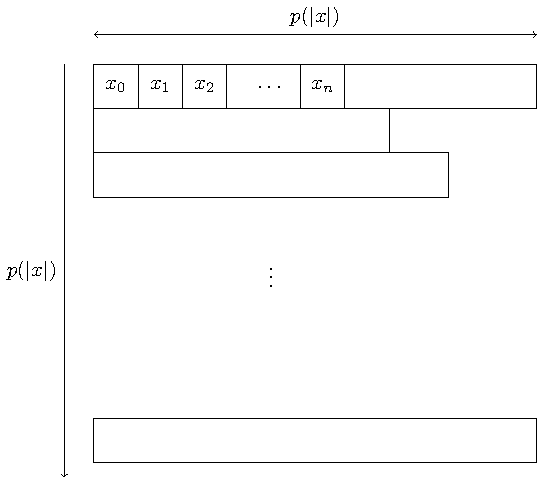
\includegraphics{./img/NPClass/SATproof1.pdf}
            \caption{Possiamo descrivere le possibili computazioni di una MdTN $M$ mediante una
            tabella così fatta.}
        \end{center}
    \end{figure}

    Vogliamo descrivere questa matrice con una formula proposizionale. Questa matrice non è unica,
    dato che esistono varie computazioni. La prima riga è fissata alla configurazione iniziale, e
    l'ultima da quella finale. Lasciamo la libertà alla matrice di rappresentare varie
    computazioni, dato che una riga non è deterministicamente determinata da quella che la precede.

    %Slide 121

    Come rappresentiamo la matrice con una formula proposizionale?
    %Abbiamo a disposizione tutte le variabili che vogliamo.
    Usiamo delle variabili $y_{i,j,x}$. $i$ rappresenta il tempo (il passo $i$ della computazione),
    $j$ corrisponde alla cella, e $x$ al simbolo dell'alfabeto della matrice che sta nella cella $j$
    al tempo $i$.  La variabile è vera se $x$ è nella cella $j$ al tempo $i$, e falsa altrimenti.
    Vogliamo ora costruire un sistema di vincoli che corrisponde all'esistenza di una computazione
    accettante che utilizzi questo tipo di variabili. Per esprimere questi vincoli usiamo delle
    formule proposizionali.

    Definiamo le ``cornici'' della matrice: prima e ultima configurazione, e i due lati della
    matrice. Possiamo supporre che il riconoscimento, se avviene, avvenga esattamente al momento
    $p(|x|)$. È facile imporre questo vincolo anche su computazioni che accettano prima. L'alfabeto
    che stiamo considerando per questa matrice è l'alfabeto $\Gamma = \Gamma \cup (Q \times
    \Gamma)$, dove $\Gamma$ è l'alfabeto di $M$ e la seconda parte codifica lo stato interno e la
    posizione della testina. Dove sta la coppia $q,x$ è posizionata la testina. Inoltre abbiamo che
    lo stato interno è $q$. Poichè stiamo lavorando con un solo nastro ci aspettiamo che la
    testina sia su un solo carattere in ogni istante della computazione.

    Perché vogliamo definire il bordo? Per semplicità. È abbastanza importante definirlo.
    %Supponiamo che $x = x_{1}\dotsc x_{n}$.
    Vogliamo che i bordi non siamo oltrepassati: li settiamo a blank e
    faremo in modo che rimangano blank per il resto della computazione.

    \begin{figure}[h]
        \begin{center}
            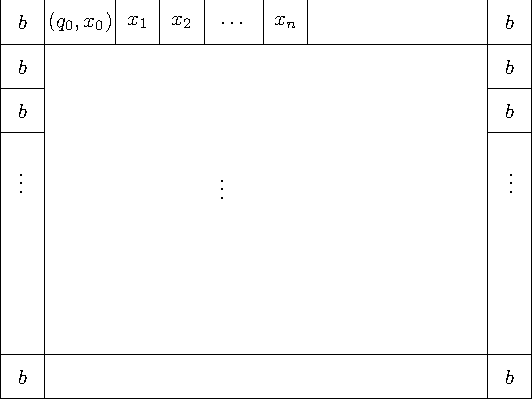
\includegraphics{./img/NPClass/SATproof2.pdf}
            \caption{Facciamo in modo che i bordi della tabella abbiano sempre il simbolo blank e
            che la prima riga corrisponda alla configurazione iniziale di $M$.}
        \end{center}
    \end{figure}

    %Slide 122

    Possiamo iniziare a definire qualche vincolo. Vogliamo che ogni cella della matrice contenga uno ed
    un solo carattere. Questo vincolo è espresso dalla seguente formula proposizionale:
    \begin{equation*}
        \phi_{0} = \bigwedge_{i=0}^{p(n)}\bigwedge_{j=0}^{p(n)}\left(\bigvee_{a \in \Gamma}
            y_{i,j,a}
        \land \bigwedge_{a,b \in \Gamma,a \not= b}(\lnot y_{i,j,a} \lor \lnot y_{i,j,b})\right)
    \end{equation*}
    
    Per ogni istante di tempo da $i$ a $p(n)$, per ogni cella da $j$ a $p(n)$ almeno una delle
    variabili $y_{i,j,a}$ deve avere valore true. La dimensione della formula è quadratica, ma per
    noi va bene perché è polinomiale. Vogliamo che tutte queste formule siano polinomiali in
    dimensione. La seconda parte del vincolo corrisponde a esprimere il fatto che vogliamo che una
    sola variabile abbia valore true tra le varie $y_{i,j,a}$ con $i$ e $j$ fissati.

    Questo vincolo è un vincolo di ``soundness'' sulla matrice. Vogliamo ora esprimere il vincolo che
    sui bordi ci siano i caratteri blank. Questo è espresso dalla seguente formula:
    \begin{equation*}
        \phi_{1} = \bigwedge_{i=0}^{p(n)}(y_{i,0,B} \land y_{i,p(n)+1,B})
    \end{equation*}

    Vogliamo fissare la configurazione iniziale e quella finale. Sappiamo com'è fatta la configurazione
    iniziale, ed esprimiamo il vincolo che la matrice esprima quella configurazione nella prima riga con
    la seguente formula:
    \begin{equation*}
        \phi_{2} = y_{0,1,(q_{0},x_{0})} \land \bigwedge_{j=2}^{n}(y_{0,j,x_{j}}) \land
        \bigwedge_{j=n+1}^{p(n)}y_{i,j,B}
    \end{equation*}

    Ci aspettiamo che il carattere 0 sia $(q,x_{0})$, che nelle restanti celle ci siano i simboli
    dell'input, e che tutte le celle da $n$ in poi siano blank.

    Ci aspettiamo poi che l'ultima riga della matrice sia una configurazione di accettazione.
    Vogliamo ovvero che corrisponda ad una configurazione finale, ovvero che da qualche parte sul
    nastro la testina si sia arrestata in uno stato di accettazione. In termini della matrice ci
    aspettiamo che nell'ultima riga ci sia una cella con un carattere $F \times \Gamma$, dove $F$
    rappresenta il sottoinsieme di $Q$ di stati accettanti. Questo è espresso dalla seguente
    formula:
    \begin{equation*}
        \phi_{3} = \bigvee_{j={1}}^{p(n)}\bigvee_{a \in F \times \Gamma}(y_{p(n),j,a})
    \end{equation*}

    Ci resta da descrivere la parte interna della matrice. In che modo vogliamo descrivere questa
    matrice? Come saranno fatte due righe successive? Saranno quasi identiche, dato che sono due
    configurazioni successive della computazione di $M$. Il nastro, durante un passo di
    computazione, cambia poco, dato che le operazioni tipiche di una MdT sono la scrittura di un
    carattere, lo spostamento della testina e il cambio del proprio stato interno. Supponiamo che la
    testina sia in una posizione $j$ con stato $q$ e carattere $a$. Cosa rimarrà sicuramente
    indentico nella riga successiva? Tutte le celle prima la cella $j-1$ e tutte le celle successive
    alla $j+1$. Al più cambiano 6 celle, in base alla riscrittura del carattere e al movimento
    della testina. 

    \begin{figure}[h]
        \begin{center}
            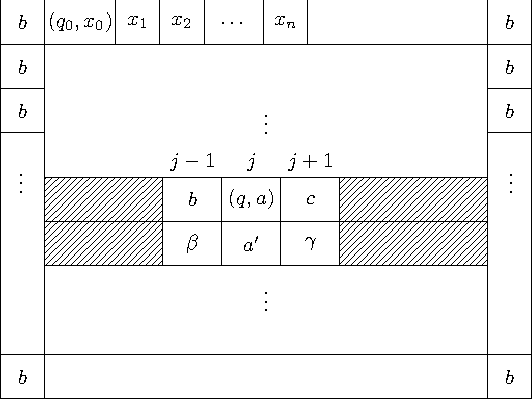
\includegraphics{./img/NPClass/SATproof3.pdf}
            \caption{Le uniche celle che cambiano durante un passo di computazione sono le 6 celle
                che comprendono quella con la testina e le altre 5 adiacenti. Avremo che $\beta = b$ e
                $\gamma = (q,c)$ se la testina si muove a destra, oppure $\beta = (q,b)$ e $\gamma = c$
            se la testina si muove a sinistra.}
        \end{center}
    \end{figure}
    %Slide 123

    Esprimiamo questo con la seguente formula:
    \begin{equation*}
        \phi_{4} = \bigwedge_{i=0}^{p(n)-1}\bigwedge_{j=1}^{p(n)}\bigwedge_{a,b,c\in \Gamma}
        (y_{i,j-1,a} \land y_{i,j,b} \land y_{i,j+1,c} \implies y_{i+1,j,b})
    \end{equation*}
    Sappiamo che, se su una cella $j$ non c'e la testina e la testina non è né nella cella $j-1$
    né in quella $j+1$ allora il carattere in $j$ non cambia.  Questo vale per tutte le celle.

    Finora non abbiamo usato molto della Macchina di Turing. Queste condizioni dipendenvano
    dall'alfabeto della macchina, dagli stati e dall'input. Quello che vogliamo ora esprimere
    dipende dalla funzione di transizione di $M$.

    La seguente formula richiede che per tutte le celle prima dell'ultima riga valga una certa
    formula $\Delta$, che andiamo a definire, e che dipende anche dai simboli di $Q \times F$:
    \begin{equation*}
        \phi_{5} = \bigwedge_{i=0}^{p(n)-1}\bigwedge_{j=1}^{p(n)}\bigwedge_{(q,a)\in Q\times F}
        \Delta_{q,a,i,j}
    \end{equation*}

    %Slide 124

    $\Delta_{q,a,i,j}$ è una formula implicativa. Supponiamo che al tempo $i$ in posizione $j$ ci
    sia la testina ed un carattere $a$, ovvero supponiamo che $y_{i,j,(q,a)}$ sia vera. Supponiamo
    inoltre che siano vere $y_{i,j-1,b}$ e $y_{i,j+1,c}$. Cosa possiamo dire di come sarà fatto il
    nastro al prossimo passo? Dipende dal programma. Consideriamo un caso particolare. Supponiamo
    che, con stato $q$ e carattere $a$, la funzione di transizione abbia due possibilità:
    \begin{equation*}
        \delta(q,a) = \set{(q',a',R),(q'',a'',L)}
    \end{equation*}
    In generale potremmo avere un numero finito diverso di possibilità. Supponiamo che la macchina non
    deterministica scelga la prima strada. Ci aspettiamo allora che $y_{i+1,j-1,b} \land y_{i+1,j,a'}
    \land y_{i+1,j+1,(q',c)}$. Questà è una possibilità. Ci aspetteremmo quindi che valga questa oppure
    $y_{i+1,j-1,(q'',b)} \land y_{i+1,j,a''} \land y_{i+1,j+1,c}$. In generale ci aspettiamo un or tra le
    possibilità. 
    %Nel caso generale avremo un or tra tutte le possibilità. 
    La formula $\Delta$ nel caso generale è così fatta:
    \begin{align*}
        \Delta_{q,a,i,j} &= \bigwedge_{b,c \in \Gamma}( y_{i,j-1,b} \land y_{i,j,(q,a)} \land
        y_{i,j+1,c} \\ &\implies \bigvee_{(q',a',M) \in \delta(q,a)}(y_{i+1,j-1,\beta_{M,q',b}} \land
        y_{i+1,j,a'} \land y_{i+1,j+1,\gamma_{M,q',c}}))
    \end{align*}
    dove
    \begin{equation*}
        \beta_{M,q',b} =
        \begin{cases}
            \case{(q',b)}{se $M = L$}\\
            \case{b}{altrimenti}\\
        \end{cases}
    \end{equation*}
    e
    \begin{equation*}
        \gamma_{M,q',c} =
        \begin{cases}
            \case{(q',c)}{se $M = R$}\\
            \case{c}{altrimenti}\\
        \end{cases}
    \end{equation*}

    Se c'è una computazione accettante la formula $\phi_{x}^{M,p} = \phi_{0} \land \phi_{1} \land
    \phi_{2} \land \phi_{3} \land \phi_{4} \land \phi_{5}$ è soddisfacibile. Viceversa se questa
    formula è soddisfacibile allora $M$ era in grado di seguire una computazione che l'avrebbe
    portata al riconoscimento della stringa. Di conseguenza abbiamo che $A \leq_{p} SAT$. L'unico
    vincolo che abbiamo sul numero e sulla dimensione delle formule è un vincolo di tipo
    polinomiale. Questa condizione è però facilmente verificata. Questo conclude la dimostrazione.

\end{proof}

Con le formule proposizionali riusciamo a descrivere una cosa complessa come una computazione di una
MdTN. In generale con formule proposizionali possiamo esprimere e modellare molte cose, da cui le
tante riduzioni a $\SAT$ o $3\SAT$.

Quando abbiamo un problema $B$ $\NPClass$-completo è interessante aggiungere vincoli per capire se
$B$ rimane $\NPClass$-completo. Ad esempio abbiamo visto che la 3-colorabilità è
$\NPClass$-completo, mentre la 2-colorabilità è in $\PClass$. A volte riusciamo ad aggiungere
abbastanza vincoli da restringerci da un problema $\NPClass$-completo ad un prolema in $\PClass$.

Sappiamo che le formule proposizionali possono essere espresse in delle forme normali. Le forme
normali tipiche sono la congiuntiva e disgiuntiva.  Una formula è in forma normale congiuntiva
(Conjunctive normal form, CNF) se può essere espressa come una congiunzione di clausole, dove la
clausole sono disgiunzioni di letterali. Un letterale è una variabile proposizionale o la sua
negata. Possiamo esprimere una clausola $A \land \lnot A \land C$ con una notazione insiemistica
come $\set{A,\lnot A,C}$. Questo perché l'or è idempotente: $A \lor A \equiv A$. Possiamo inoltre
rappresentare una conginzione di congiunzioni con una notazione insiemistica, come ad esempio
$\set{\set{A,\lnot A,C},\set{A,\lnot B}}$.

Che vincoli possiamo immaginare di porre a $\SAT$? Possiamo immaginare di dare un vincolo al numero
di letterali nelle clausole. Se poniamo un vincolo di 3 letterali in ogni clausola otteniamo
$3\SAT$, l'insieme delle formule soddisfacibili espresse in CNF con clausole di 3 letterali.

Otteniamo in questo modo un problema più semplice di $\SAT$? Vedremo che in realtà no, poichè
$\SAT \leq 3\SAT$.

\section{Riduzioni di problemi $\NPClass$-completi}

\subsection{$\SAT \leq 3\SAT$}

%Siamo ora interessati ad una ``restrizione'' di $\SAT$: $3\SAT$.

\begin{thm}
        $\SAT \leq 3\SAT$.
\end{thm}

Mostriamo ora che $3\SAT$ è $\NPClass$-completo mostrando una riduzione da $\SAT$ a $3\SAT$. Per
fare ciò ci serve una trasformazione che richiede tempo polinomiale da formule generali a formule
in 3-CNF tale che conservi la soddisfacibilità della formula.

Quando vogliamo facciamo una trasformazione di una formula di solito vogliamo ottenere una formula
equivalente a quella di partenza. In questo caso a noi interessa una cosa più debole: ottenere una
formula che sia soddisfacibile sse la formula di partenza era soddisfacibile.

Vediamo perché non ci conviene usare una trasformazione che ci permtte di passare ad una formula
logicamente equivalente a quella di partenza. Data una qualsiasi formula della logica proposizionale
possiamo trasformarla in una logicamente equivalente in forma normale congiuntiva. Possiamo fare
questo perché esistono varie equivalenze logiche notevoli che ci permettono di dare alla formula la
forma che desideriamo: ad esempio, $A \implies B \equiv \lnot A \lor B$.

Il primo passaggio è trasformare tutti i connettivi nelle formule in loro corrispettivi equivalenti
espressi con $\lor,\land,\lnot$. Dopodiché ``pushiamo'' le negazioni al più interno possibile nella
formula. Le regole che ci permettono di propagare la negazione all'interno della formula sono le
formule di de Morgan: ad esempio $\lnot (A \land B) \equiv \lnot A \lor \lnot B$. La propagazione
della negazione si blocca quando giungiamo alle formule atomiche. Abbiamo ancora un nesting
arbitrario di congiunzioni e disgiunzioni però. Questo può essere risolto utilizzando le regole di
distributività: ad esempio, $A \lor (B \land C) \equiv (A \lor B) \land (A \lor C)$.

In questo modo possiamo ottenere una formula equivalente in 3-CNF. Abbiamo però un problema
abbastanza grave: in generale questa trasformazione può portare ad una esplosione esponenziale
della dimensione della formula. Questa trasformazione richiede quindi tempo esponenziale, e di
conseguenza non si tratta di una riduzione polinomiale.

Noi però siamo interessati alla soddisfacibilità. Se non siamo interessati a preservare
l'equivalenza logica possiamo usare una trasformazione che conserva la soddisfacibilità e che non
porta ad un'esplosione esponenziale.

Vediamo questa trasformazione con un esempio. Prendiamo la formula seguente:
\begin{equation}\label{eq:start}
    \bigvee_{i=1}^{n}(x_{i}\land y_{i}) = (x_{1} \land y_{1}) \lor \cdots \lor (x_{n} \land y_{n})
\end{equation}

Se la trasformassimo in una formula equivalente utilizzando il metodo appena descritto otterremmo le
$2^{n}$ clausole:
\begin{equation*}
    \set{x_{1},\dotsc,x_{n-1},x_{n}},\set{x_{1},\dotsc,x_{n-1},y_{1}},\dotsc,\set{y_{1},\dotsc,y_{n-1},y_{n}}
\end{equation*}

Se invece passiamo dalla formula di partenza alla seguente, espressa come insieme di clausole:
\begin{equation}\label{eq:transformation}
    \set{z_{1},\dotsc,z_{n}},\set{\lnot z_{1},x_{1}},\set{\lnot z_{1},y_{1}},\dotsc,\set{\lnot
    z_{n},x_{n}},\set{\lnot z_{n},y_{n}}
\end{equation}
Otteniamo una formula soddisfacibile se e solo se lo era quella di partenza, ma che non è ad essa
logicamente equivalente.  Inoltre la dimensione aumenta in modo lineare.  Ogni $z_{i}$ ci indica se
la coppia $x_{i} \land y_{i}$ era vera.

Se introduciamo variabili diverse due formule non possono essere equivalenti. Le equivalenze si
stabbiliscono tra formule con le stesse variabili.

Se la formula \ref{eq:transformation} è vera almeno uno $z_{i}$ deve essere vero. In più tutte le
altre clausole devono essere vere. Dove $z_{i}$ è vero sia $x_{i}$ che $y_{i}$ devono essere veri.
Ma allora era vera anche la formula \ref{eq:start}.

Adottando questa tecnica è possibile dimostrare che ogni formula proposizionale può essere
trasformata in 3-CNF preservando la soddisfacibilità con una crescità al più polinomiale.

In generale non è vero che possiamo trasformare una formula in una equivalente in CNF in tempo
polinomiale. Se siamo interessati alla soddisfacibilità possiamo fare una trasformazione
polinomiale che ci restituisce una formula ``soddsifacibilmente equivalente'' a quella di partenza.
In particolare quest'ultima trasformazione non preserva la tautologicità di una formula.

\subsection{$3\SAT \leq \VC$}

Vediamo ora un teorema abbastanza importante. È un esempio interessante di riduzione. Vogliamo
dimostrare che $3\SAT$ è riducibile a $\VC$.

\begin{thm}
        $3\SAT \leq \VC$
\end{thm}

Ricordiamo che $\VC$ è il problema del ricoprimento di vertici:
\begin{equation*}
    \VC = \set{\pair{G}{k} \mid \text{Esiste un ricoprimento di vertici in $G$ di dimensione $\leq k$}}
\end{equation*}

Un ricoprimento di vertici è un sottoinsieme $S$ di $V$ tale che per ogni arco uno dei nodi
dell'arco ricade in $S$.

Sono due problemi a priori diversi. Ci si potrebbe chiedere cosa abbia a che fare l'uno con l'altro.
Le riduzioni, in genere, mettono in relazione mondi diversi: ci permettono di vedere vari problemi
in modi diversi ma equivalenti.

La prima cosa da chiedersi quando si vuole fare una riduzione è cosa richiedono in input il primo e
il secondo problema. $3\SAT$ richiede una formula $\varphi$ in 3-CNF e decide se questa è
soddisfacibile o meno. Vertex Cover prende in input un grafo $G$ ed un intero $k$. La $f$ che
vogliamo costruire prende in input la formula $\varphi$ e restituisce in output una coppia
$\pair{G}{k}$. Inoltre vogliamo che $f \in \FP$.
\begin{equation*}
    \varphi \overset{f}{\mapsto} \pair{G}{k}
\end{equation*}

Dobbiamo inoltre dimostrare che $\varphi \in 3\SAT \iff \pair{G}{k} \in \VC$. La definizione di $f$
richiede del lavoro creativo.

Partiamo da un esempio. Supponiamo di avere una formula così fatta:
\begin{equation*}
    \phi = \set{\set{A,\lnot B, C},\set{\lnot A, B \lnot C},\set{\lnot A,\lnot B, C},\set{A,B,\lnot
    C}}
\end{equation*}

Questa formula è soddisfacibile. Se prendessimo la congiunzione di tutte le 8 possibili clausole la
formula sarebbe insoddisfacibile. È facile verificare che qualsiasi sottoinsieme stretto delle
possibili clausole sarebbe soddisfacibile. Questo ci mostra che nonostante $3\SAT$ sia un problema
$\NPClass$-completo possono esistere delle euristiche che ci aiutano a capire se una formula è
soddisfacibile o meno in maniera efficiente per certi casi particolari.

Da questa formula dobbiamo ottenere un grafo ed assegnargli un $k$. Il grafo $G$ è fatto così:
\begin{itemize}
        \item Colleghiamo con un arco ogni letterale con il suo negato, creando un insieme di coppie
        \item Creiamo dei ``triangoli'' per ogni clausola
        \item Colleghiamo i letterali tra di loro tra le coppie e i triangoli
\end{itemize}
La costruzione è rappresentata nelle figure \ref{img:SATtoVC1} e \ref{img:SATtoVC2}

\begin{figure}[h]
    \begin{center}
        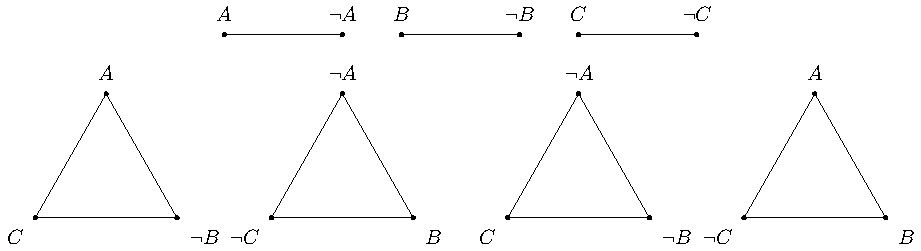
\includegraphics[scale=0.75]{./img/NPClass/SATtoVC1.pdf}
        \caption{Strutture di base del grafo $G$: coppie e triangoli.}
        \label{img:SATtoVC1}
    \end{center}
\end{figure}

\begin{figure}[h]
    \begin{center}
        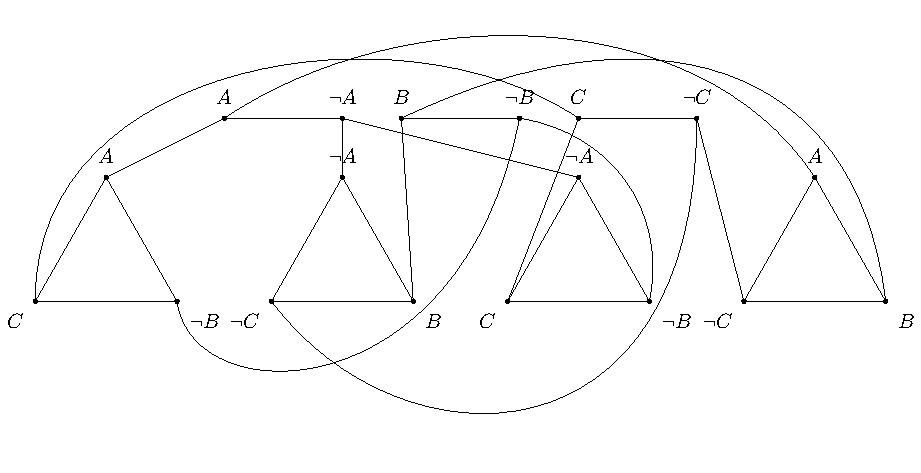
\includegraphics[scale=0.75]{./img/NPClass/SATtoVC2.pdf}
        \caption{Aggiunta degli archi tra i vertici del grafo.}
        \label{img:SATtoVC2}
    \end{center}
\end{figure}

Quanti sono i nodi del grafo? Supponiamo che $n$ sia il numero delle variabili ed $m$ il numero
delle clausole. Per il nostro esempio $n=3$ e $m=4$. Abbiamo che il numero di nodi è $2n + 3m$.

È un grafo abbastanza sparso. Potremmo contare gli archi, ma è abbastanza evidente che questi
siano in numero lineare nel numero dei nodi.

Quanti nodi dobbiamo prendere per coprire tutti gli archi? Per i triangoli almeno 2; per le coppie
almeno 1. Un ricoprimento deve avere una dimensione minima $2m + n$. Questo sarà il nostro $k$
della riduzione. Abbiamo quindi la nostra trasformazione $f$. Vogliamo dimostrare che se questo
grafo ha un ricoprimento di cardinalità $\leq k$ la formula di partenza è soddisfacibile, e
viceversa.

Mostriamo i due versi del sse, che sono abbastanza diversi.

Supponiamo che $\varphi$ sia soddisfacibile. Esiste quindi un'assegnamento di valori di verità che
rende la formula soddisfacibile. Nel nostro esempio andrebbe bene l'assegnamento che assegna falso a
tutte le variabili proposizionali. Nel nostro grafo nelle coppie scegliamo per il ricoprimento il
letterale che, in base all'assegnemento, ha valore vero. In questo caso prenderemmo $\lnot A, \lnot
B, \lnot C$. Nei triangoli delle clausole abbiamo che c'è un letterale direttamente collegato ad
uno dei letterali già scelti. Ad esempio, nel primo triangolo abbiamo che $\lnot B$ è collegato al
corrispondente nella seconda coppia. Questo arco tra i due $\lnot B$ è gia coperto. Di conseguenza
scegliamo per il ricoprimento gli altri due nodi. Facciamo questo per ogni clasuola. Quello che
otteniamo è un ricoprimento su $G$ di dimensione $2m + n$. Quindi se $\varphi$ è soddisfacibile
esiste un ricoprimento di dimensione $\leq k$.

Prendiamo ora il verso opposto. Supponiamo esista un ricoprimento di dimensione $2m + n$. Se abbiamo
un tale ricoprimento abbiamo che per ogni triangolo abbiamo preso almeno due vertici e per ogni
coppia abbiamo preso uno dei vertici. Per l'assegnamento dei valori di verità assegnamo valore vero
ai vertici presi dalle coppie. Abbiamo che uno dei nodi, per ogni triangolo, deve toccare uno dei
nodi che abbiamo selezionato nelle coppie. Di conseguenza tale assegnamento di valori di verità
soddisfa la formula. Di conseguenza se esiste un ricoprimento di dimensione $2m + n$ abbiamo che la
$\varphi$ corrispondente è soddisfacibile.

\begin{figure}[h]
    \begin{center}
        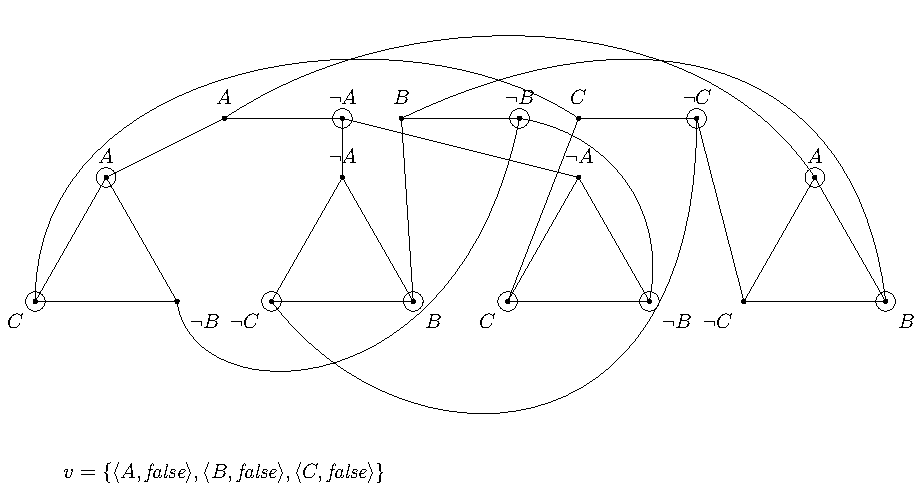
\includegraphics[scale=0.75]{./img/NPClass/SATtoVC3.pdf}
        \caption{I nodi cerchiati nel grafo $G$ fanno parte del sottoinsieme $S$ di copertura dei
        vertici.}
    \end{center}
\end{figure}

Questo ci mostra, nuovamente, quanto siano importanti i grafi in informatica: sono una struttura
dati flessibile che ci permette di modellare molti problemi. Molti di questi possono essere espressi
come problemi di visita su grafi.

Abbiamo già visto che $\VC$ è equivalente al problema della cricca e al problema dell'insieme
indipendente. Di conseguenza, poichè abbiamo che $\VC$ è $\NPClass$-completo per la dimostrazione
appena vista, abbiamo che anche cricca e insieme indipendente sono problemi $\NPClass$-completi.

\subsection{$\HAMPATH \equiv \HAMCYCLE$}

Vediamo una riduzione dal problema del cammino hamiltoniamo al ciclo hamiltoniano e una riduzione
inversa. Questi due problemi sono equivalenti.

Quello che vogliamo per ridurre il cammino hamiltioniano al ciclo hamiltoniano è una riduzione tra
grafi che ci porti dal problema dell'esistenza di un cammino hamiltioniano al problema
dell'esistenza di un ciclo hamiltoniano.

Quello che facciamo è aggiungere un nodo collegato a tutti i nodi del grafo $G$ di partenza.

\begin{figure}[h]
    \begin{center}
        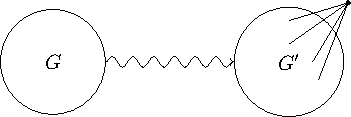
\includegraphics{./img/NPClass/HAMPATHCYCLE.pdf}
        \caption{Aggiungendo un nodo collegato a tutti gli altri trasformiamo un qualsiasi cammino
        hamiltoniano esistente in $G$ in un circuito che passa per il nuovo nodo.}
    \end{center}
\end{figure}

Se abbiamo un cammino hamiltoniano in $G$ otteniamo un ciclo in $G'$ passando per il nuovo nuovo $n$
aggiunto dall'ultimo nodo del cammino e passando al primo nodo del cammino. Viceversa, se abbiamo un
ciclo in $G'$ questo include necessariamente $n$. Togliendo $n$ dal ciclo otteniamo un cammino
hamiltoniano in $G$.

L'altro verso è più complesso. Non basta l'identità come trasformazione perché con questa non
vale il sse. L'identità serve in genere a ridurre un problema a se stesso.

L'idea è la seguente: partendo dal grafo selezioniamo un nodo arbitrario $n$. Questo nodo avrà un
pò di connessioni con altri nodi. Costruiamo una copia di questo nodo: aggiungiamo un nodo nuovo
$n'$ collegato a tutti i nodi a cui era collegato $n$. Aggiungiamo poi due nuovi nodi $m,m'$
collegati, rispettivamente, a $n$ e $n'$.

Il grafo $G'$ così costruito a partire da $G$ ha un cammino hamiltoniano sse $G$ aveva un ciclo
hamiltoniano. Infatti sia $n$ il nodo che viene ``clonato'' in $G$ e sia $p = n_{1}, \dotsc,
n_{i-1}, n, n_{i}, \dotsc, n_{n}, n_{1}$ un ciclo hamiltoniano in $G$. In $G'$ costruiamo un cammino
hamiltoniano a partire da $p$ nel seguente modo: partiamo da $m$, passiamo per $n$, e seguiamo $p$
in un qualche verso. Ad esempio da $n$ passiamo a $n_{i}$ fino a tornare a $n_{i-1}$. A questo punto
da $n_{i-1}$ passiamo al nodo clone $n'$ e da lì passiamo infine ad $m'$. Possiamo passare da
$n_{i-1}$ a $n'$ poichè $n'$ è collegato a tutti i nodi adiacenti ad $n$, e $n_{i-1}$ è adiacente
ad $n$.

Viceversa, se in $G'$ abbiamo un cammino hamiltoniano allora abbiamo un circuito hamiltoniano in
$G$. Infatti se esiste un cammino hamiltoniano $p'$ questo deve necessariamente avere come estremi
del cammino $m$ e $m'$. Sia, ad esempio, $p' = m, n, n_{i},\dotsc, n_{i-1}, n', m'$. Da $p'$
possiamo ottenere un ciclo hamiltoniano in $G$ nel seguente modo: da $p'$ rimuoviamo $m, n'$ e $m'$
e aggiungiamo $n$ in fondo per chiudere il circuito. Siamo sicuri che questo sia un circuito
hamiltoniano in $G$ poichè se $n_{i-1}$ era adiacente a $n'$ allora necessariamente era adiacente
anche ad $n$.

Illustriamo questa trasformazione con l'esempio in figura \ref{img:HAMCYCLEPATH}.

\begin{figure}[h]
    \begin{center}
        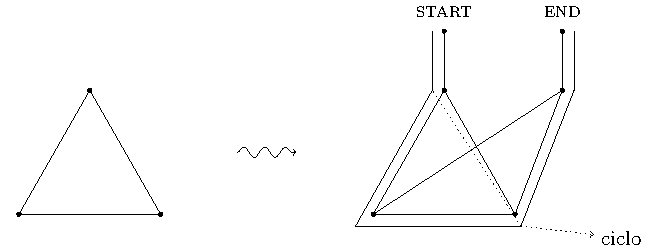
\includegraphics{./img/NPClass/HAMCYCLEPATH.pdf}
        \caption{Da un ciclo hamiltoniano in $G$ passiamo ad un cammino hamiltoniano in $G'$ e,
        viceversa, da un cammino hamiltoniano in $G'$ passiamo ad un ciclo in $G$.}
        \label{img:HAMCYCLEPATH}
    \end{center}
\end{figure}

\subsection{$\HAMPATH \leq \HAMPATH_{u,v}$}

Vediamo ora una riduzione dal problema del cammino hamiltioniano al problema del cammino
hamiltonianio puntato, che consiste nel trovare, se esiste, un cammino hamiltoniano in un grafo $G$
tra due nodi $u, v$ dati in input.

Apparentemente il secondo sembrerebbe più semplice del primo. In realtà ciò non è vero, poichè
esiste una riduzione dal primo al secondo.

La trasformazione $f$ funziona così: dato un grafo $G$ si crea un grafo $G'$ aggiundendo due nuovi
nodi $n_{\textsc{start}}$ e $n_{\textsc{end}}$ e degli archi da tutti i nodi di $G$ a
$n_{\textsc{start}}$ e $n_{\textsc{end}}$. Il risultato della trasformazione $f$ applicata a $G$ è
la tripla $\tuple{G',n_{\textsc{start}},n_{\textsc{end}}}$.

Mostriamo ora che la riduzione data è corretta. Supponiamo esista un cammino hamiltoniano $p$ in
$G$. Allora esiste anche un cammino hamiltoniano puntato da $n_{\textsc{start}}$ a
$n_{\textsc{end}}$ in $G'$. Infatti è possibile estendere $p$ aggiungendo $n_{\textsc{start}}$ e
$n_{\textsc{end}}$ alla fine. Ciò è possibile perché sia $n_{\textsc{start}}$ che
$n_{\textsc{end}}$ sono collegati a tutti i nodi di $G$, e in particolare sono anche collegati agli
eventuali estremi di un cammino hamiltoniano in $G$.

Viceversa, supponiamo in $G'$ esista un cammino hamiltoniano $p'$ puntato da $n_{\textsc{start}}$ a
$n_{\textsc{end}}$. Da $p'$ possiamo ottenere un cammino hamiltoniano $p$ per il sottografo di $G'$
che corrisponde a $G$ semplicemente rimuovendo $n_{\textsc{start}}$ e $n_{\textsc{end}}$.

È inoltre facile verificare che la trasformazione $f$ richiede tempo polinomiale.

\begin{figure}[h]
    \begin{center}
        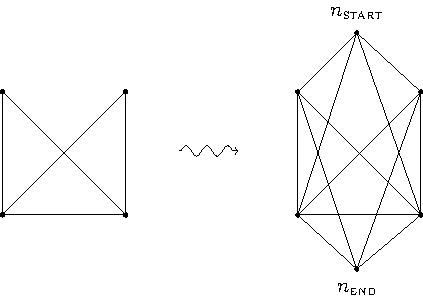
\includegraphics{./img/NPClass/HAM2PHAM.pdf}
        \caption{Esempio di riduzione da $\HAMPATH$ a
        $\HAMPATH_{n_{\textsc{start}},n_{\textsc{end}}}$.}
    \end{center}
\end{figure}

\subsection{$\SAT \leq \dHAM$}

Vediamo ora un'altra riduzione classica e non del tutto ovvia.

Questa ci permette di dimostrare che l'esistenza di un cammino hamiltoniano è un problema
$\NPClass$-completo. Lo dimostreremo nel caso di grafi orientati, ma in realtà e dimostrabile anche
per grafi non orientati.

$\dHAM$ è il problema decisionale dell'esistenza di un cammino hamiltoniano in un grafo orientato.

Vediamo la riduzione per un esempio semplice. Il procedimento è tuttavia generale e vale per
qualsiasi formula in forma a clausole (senza vincoli sul numero di letterali nelle clausole).

Consideriamo la formula proposizionale $\varphi$ espressa dalla congiunzione delle due clausole
$\set{A,B}$ e $\set{\lnot A}$.

Costruiamo un grafo diretto $G$ a partire da $\varphi$ in cui esiste un cammino hamiltoniano sse la
$\varphi$ è soddisfacibile. In $\varphi$ abbiamo 2 clausole e 2 variabili proposizionali. Per ogni
variabile proposizionale costruiamo una catena con 6 nodi. 2 di questi rappresentano le estremità
della catena e ogni coppia di nodi consecutivi nella catena (escludendo gli estremi) corrisponde ad
una clausola.  Nel caso generale in cui $\varphi$ ha $m$ clausole e $n$ variabili costruiremmo $n$
catene, con $2m + 2$ nodi ciascuna. 

Su ciascuna catena fissiamo due versi di attraversamento, aggiungendo, per ogni coppia di nodi della
catena (estremi inclusi) una coppia di archi: un arco dal primo al secondo ed un arco dal secondo al
primo.

Concettualmente ad ogni clausola è associata una ``colonna'', ovvero una coppia di nodi ``interna''
alla catena.

\begin{figure}[h]
    \begin{center}
        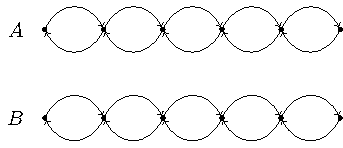
\includegraphics{./img/NPClass/SATdHAM1.pdf}
        \caption{Costruzione delle catene nella riduzione da $\SAT$ a $\dHAM$.}
    \end{center}
\end{figure}

Aggiungiamo un nodo di partenza e uno di arrivo. Dal nodo di partenza aggiungiamo due archi, uno che
va al nodo iniziale della catena di $A$ e uno che va al nodo finale della stessa catena. Dagli
estremi della catena di $B$ aggiungiamo due archi che vanno al nodo di arrivo. Colleghiamo poi le
catene in cascata, aggiungendo da entrambi i nodi all'estremità di una catena degli archi che vanno
alle estremità della catena successiva. L'idea è che nel percorrere una catena possiamo uscire da
uno qualsiasi dei due lati, e quando usciamo vogliamo passare a quella successiva.

\begin{figure}[h]
    \begin{center}
        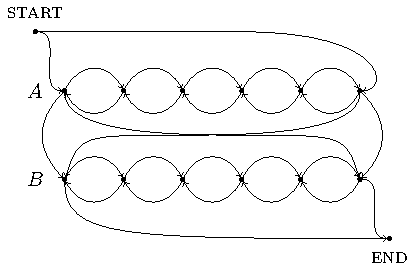
\includegraphics{./img/NPClass/SATdHAM2.pdf}
        \caption{Aggiunta di nodi di partenza/arrivo e link tra questi e le catene e tra le catene.}
    \end{center}
\end{figure}

Aggiungiamo poi un nodo per ogni clausola. Il verso di attraversamento di una catena in un cammino
hamiltoniano in $G$ ci dirà quale sarà il valore di verità associato alla variabile a cui la
catena fa riferimento. Inoltre nell'attraversare le catene vogliamo ``toccare'' la clausola che
viene soddisfatta da quell'assegnamento di verità. Supponiamo di avere una clausola $a$ che
contiene $A$. Aggiungiamo quindi nella catena di $A$ un arco dal nodo di sinistra della colonna
associata ad $a$ al nodo di $a$ ed un link dal nodo di $a$ al nodo di destra della colonna associata
ad $a$. Per le clausole $a'$ che contengono $\lnot A$ aggiungiamo un arco dal nodo di destra della
colonna associata ad $a'$ al nodo di $a'$ e aggiungiamo un arco dal nodo di $a'$ al nodo di sinistra
della colonna associata ad $a'$.

\begin{figure}[h]
    \begin{center}
        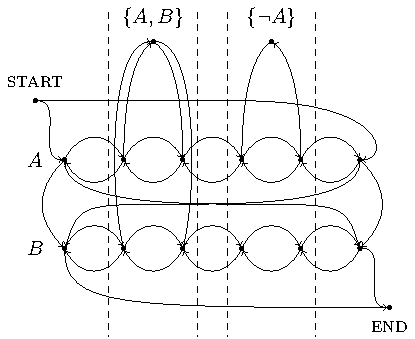
\includegraphics{./img/NPClass/SATdHAM3.pdf}
        \caption{Aggiunta dei nodi delle clausole e dei relativi link.}
    \end{center}
\end{figure}

Se $\varphi$ è soddisfacibile allora il grafo $G$ così costruito contiene un cammino hamiltoniano,
e viceversa se $G$ ammette un cammino hamiltoniano $\varphi$ è soddisfacibile.

Infatti, supponiamo che $\varphi$ sia soddisfacibile. In tal caso abbiamo un assegnamento di valori
di verità alle variabili proposizionali che la soddisfa. Per ogni variabile $A$ attraversiamo la
catena corrispondente nel verso da sinistra a destra se $A$ ha valore \textit{true}, e in verso
opposto se $A$ ha valore \textit{false}. Inoltre nel cammino tocchiamo tutte le clausole che non
sono già state toccate.  Questo è possibile grazie ai link alle clausole. Partendo da
$\textsc{start}$, seguendo le direzioni degli assegnamenti, toccando le clausole e finendo in
$\textsc{end}$ otteniamo un cammino hamiltoniano in $G$.

Cosa ci obbliga ad attraversare una catena secondo la nostra convenzione sul verso di
attraversamento? La direzione dei link alle clausole. Se infatti, ad esempio, attraversassimo la
catena di $A$ da sinistra verso destra, ovvero in verso opposto rispetto a quello dettato dalla
convenzione sul valore di verità di $A$, non riusciremmo a toccare il nodo corrispondente alla
clasuola $\set{\lnot A}$, e non avremmo un cammino hamiltoniano.

Vediamo ora il verso opposto della riduzione, leggermente meno intuitivo. Supponiamo che $G$ abbia
un cammino hamiltoniano. Quello che vogliamo dimostrare è che se cominciamo ad attraversare una
catena in una direzione giungeremo alla fine della catena seguendo la stessa direzione. In altri
termini non possiamo ``tornare indietro'' lungo una catena.

Abbiamo sicuramente che non possiamo invertire la direzione dell'attraversamento usando gli archi
inversi tra i nodi della catena. Quello che è meno evidente è che non possiamo avere un percorso
diverso sfruttano i link alle clausole. In realtà questo non è possibile, poichè se prendiamo uno
degli archi che collega alle clausole l'unica mossa successiva possibile è quella di scendere al
nodo successivo della catena. Infatti, supponiamo di essere al nodo $n$ della catena di $A$, di
passare al nodo della clausola $\set{A,B}$ e di passare al nodo della catena di $B$.  Abbiamo che,
poichè dobbiamo passare per tutti i nodi nel cammino hamiltoniano, se mai arrivassimo al nodo $n+1$
saremmo bloccati, dato che tutti i nodi adiacenti ad $n+1$ sarebbero già stati toccati. L'unico
modo in cui si potrebbe avere un cammino hamiltoniano in questo modo è se $n+1$ fosse l'ultimo nodo
del cammino. Ma questo è impossibile, dato che, per come è fatto $G$, un qualsiasi cammino
hamiltoniano in $G$ deve necessariamente finire nel nodo $\textsc{end}$. Di conseguenza non
esisterebbe in $G$ un cammino hamiltoniano, e questo contraddice la nostra ipotesi.

Perciò in un cammino hamiltoniano $p$ in $G$ consumiamo tutte le catene una alla volta seguendo una
determinata direzione. A questo punto attribuiamo un valore di verità alle variabili proposizionali
in base alla direzione di attraversamento della catena corrispondente. Ad esempio, da sinistra a
destra corrisponde a vero e il verso opposto corrisponde a falso. Questo assegnamento soddisfa le
clausole perché le clausole devono essere toccate nel cammino $p$. Ma toccare una clausola
corrisponde a soddisfarla con un determinato assegnamento di verità ad una variabile
proposizionale.

Abbiamo che il grafo $G$ è abbastanza sparso. Abbiamo che il fattore di branching del grafo è
abbastanza piccolo. Di conseguenza è facile verificare che la dimensione del grafo è polinomiale
nella dimensione della formula. Questo ci mostra che un fattore di branching di valore costante e
basso in un grafo $G$ non semplifica il problema della ricerca di un cammino hamiltoniano in $G$.

\subsection{$\HAMPATH \leq \TSP$}

Vediamo un'altra riduzione interessante. Consideriamo il problema del commesso viaggiatore
(Traveling Salesperson Problem, $\TSP$). Abbiamo un grafo non orientato completo $G$ i cui archi
$(u,v)$ sono etichettati da un valore $d_{u,v}$. Supponiamo che la ``distanza'' $d$ sia simmetrica:
$d_{u,v} = d_{v,u}$. Ci chiediamo se esiste un cammino in $G$ che ci permette di toccare tutti i
nodi con una somma dei valori degli archi (``distanza complessiva'') minore o uguale ad un certo
$k$.

\begin{equation*}
    \TSP = \set{\tuple{G,k,d} \mid G = (V,V^{2}) \land \exists p. \sum_{(u,v)\in p}d_{u,v} \leq k}
\end{equation*}

Sappiamo già che questo problema è in $\NPClass$. Infatti esiste un certificato polinomiale per
una soluzione a questo problema: il percorso del commesso viaggiatore.

Vediamo che $\TSP$ è $\NPClass$-completo riducendo il problema del cammino hamiltoniano a $\TSP$.
Infatti dato un grafo $G$ con $n$ nodi passiamo ad un grafo completo $G'$ con i seguenti
assegnamenti di peso agli archi:
\begin{itemize}
    \item se $(u,v) \in G$, $d_{u,v} = 1$ 
    \item se $(u,v) \notin G$, $d_{u,v} = 2$ 
\end{itemize}
Come valore per $k$ scegliamo $n-1$.

Agli archi che non esistevano in $G$ diamo un peso abbastanza grande da renderli non convenienti da
attraversare. Infatti se vogliamo un cammino che tocchi tutti i nodi di distanza complessiva $n-1$
non potremmo mai passare per un arco di peso maggiore di 1.

In figura \ref{img:HAMTSP} è rappresentato un esempio con un grafo con 4 nodi.

\begin{figure}[h]
    \begin{center}
        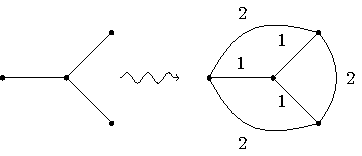
\includegraphics{./img/NPClass/HAMTSP.pdf}
        \caption{Esempio di riduzione da cammino hamiltoniano a commesso viaggiatore.}
        \label{img:HAMTSP}
    \end{center}
\end{figure}

% TODO add proof of correctness

Abbiamo quindi che $\TSP$ è NP-completo.

\subsection{$\VC \leq \HIT$}

Vediamo un'altra riduzione. Supponiamo di avere un insieme $S$ di individui. Questi sono raggruppati
in classi $A_{1},\dotsc,A_{n} \subseteq S$. Possiamo supporre che l'unione degli $A_{i}$ sia uguale
ad $S$. Ci chiediamo se esiste un insieme $H \subseteq S$ tale che $\forall i, H \cap A_{i} \not=
\emptyset$. Chiediamo inoltre che $|H| \leq k$. Questo $H$ è solitamente detto \textit{hitting
set}. L'input del problema è $S$, la famiglia $\set{A_{i}}$ e l'intero $k$.

A priori $H$ potrebbe essere un qualsiasi sottoinsieme di $S$. Potremmo quindi fare una ricerca
esaustiva per trovare $H$. Questo ci permette di definire lo spazio di ricerca, che ha dimensione
esponenziale nel numero degli elementi di $S$. Sappiamo quindi che questo problema è in $\NPClass$.
In maniera analoga potremmo trarre la stessa conclusione se pensiamo ad un semplice algoritmo di
verifica per il problema, che esiste: dato un $H$ basta verificare che ha intersezione nulla con gli
$A_{i}$ e cardinalità $\leq k$.

\begin{figure}[h]
    \begin{center}
        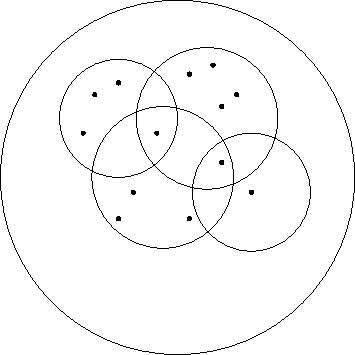
\includegraphics{./img/NPClass/HIT.pdf}
        \caption{Esempio di problema di ricerca dell'hitting set}
    \end{center}
\end{figure}

Questo problema rappresenta una generalizzazione del problema della copertura di vertici. Possiamo
pensare ad ogni sottoinsieme come ad un iperarco, ovvero un arco che collega più di due nodi.
Possiamo immaginare di avere un ``hub'' centrale che collega tutti i nodi collegati dall'iperarco
mediante archi normali.

Andando a sostituire in $S$ gli $A_{i}$ con insiemi di nodi collegati da iperarchi otteniamo un
ipergrafo, e il problema dell'hitting set si riduce alla ricerca di una copertura di vertici di
dimensione minore uguale a $k$ in questo ipergrafo.

\begin{figure}[h]
    \begin{center}
        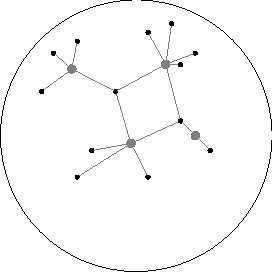
\includegraphics{./img/NPClass/HYPERGRAPH.pdf}
        \caption{Il problema dell'hitting set può essere visto come un problema di copertura di
        vertici su un ipergrafo.}
    \end{center}
\end{figure}

Vediamo quindi una riduzione da $\VC$ a $\HIT$. Supponiamo di lavorare con un grafo $G$ non
orientato.

Supponiamo di avere una coppia $(G,k) \in \VC$ e costruiamo una funzione $f$ che mappi $(G,k)$ in
$(S,\set{A_{i}},k)$. Supponendo che $G = (V,E)$, poniamo $S = V$, $\set{A_{i}} = \set{\set{u,v}
\mid (u,v) \in E}$ e $k$ rimane invariato. Intuitivamente cerchiamo un hitting set nell'insieme dei
nodi di $G$ supponendo di avere un sottoinsieme $A_{i}$ per ogni coppia di nodi $(u,v)$ di
cardinalità $\leq k$, che corrisponde ad una copertura di vertici in $G$.

% TODO add proof of correctness

\subsection{$\HAMPATH \leq k-\ST$}

Dato un grafo $G = (V,E)$ uno spanning tree $T$ è uno sottografo connesso di $G$ con gli stessi
nodi di $G$ e con $n-1$ archi. Un grafo ammette uno spanning tree se e solo se è connesso.

Esistono vari problemi al riguardo agli spanning tree su grafi. Ad esempio l'esistenza di uno
spanning tree in $G$, che si riduce a capire se il grafo è connesso, che è un problema semplice.
Infatti ogni visita del grafo definisce implicitamente uno spanning tree. 

Il problema diventa interessante se poniamo vincoli allo spanning tree. Un vincolo interessante è,
ad esempio, dare un limite $k$ al numero delle estremità dello spanning tree, ovvero dei nodi da
cui parte un unico arco nello spanning tree.

Lo spazio di ricerca del problema è grande. Esiste un algoritmo di verifica veloce: dato uno
spanning tree verifichiamo che contiene tutti i vertici e contiamo le estremità. Ci verrebbe il
sospetto che sia $\NPClass$-completo. Cerchiamo quindi un problema $\NPClass$-completo che gli
somigli. 

Se fissiamo $k$ a 2 abbiamo che lo spanning tree corrisponde ad un cammino hamiltoniano. Il cammino
hamiltoniano è quindi un ``caso particolare'' di spanning tree. Quest'ultimo problema è quindi
più complicato del problema del cammino hamiltoniano.

% TODO add proof of correctness

\subsection{$k-\CLIQUE \in \PClass$}

% ripetizione su fatto, 
Per tanti dei problemi che abbiamo visto il fatto che uno di questi sia in $\NPClass$, e che,
presumibilmente, non sia in $\PClass$, è una conseguenza del fatto che stiamo cercando un algoritmo
che lavori in maniera uniforme su input arbitrari. Ci chiediamo quindi se indebolire un problema,
mediante, ad esempio, dei vincoli sull'input, possa produrre un problema che sta in $\PClass$. La
risposta è positiva, quantomeno per certi problemi e per certi vincoli.

Prendiamo in considerazione il problema della Cricca. L'input è un grafo $G$, un intero $k$, e ci
chiediamo se esiste una cricca di dimensione $k$ in $G$. Sappiamo che, nella sua forma generale, è
un problema $\NPClass$-completo.

Supponiamo di fissare $k$ a priori, ad esempio a 7. Quello che prendiamo in input in questo caso
è solamente $G$ e ci chiediamo se esiste una cricca di dimensione 7 in $G$. Qual è la classe di
complessità a cui appartiene questo problema?

La prima cosa da fare per rispondere a questa domanda è definire lo spazio di ricerca, usando un
algoritmo banale che provi tutte le combinazioni di 7 nodi. Consideriamo tutti i possibili candidati
e li testiamo per vedere se un certo candidato è una cricca. È un algoritmo brutale, ma ci
permette di dare un upper bound allo spazio di ricerca. Supponiamo che $G=(V,E)$ e $|V| = n$.
Dobbiamo calcolare il numero di combinazioni diverse di 7 nodi. Questo valore è dato da:
\begin{equation*}
    \binom{n}{7} = \frac{n!}{(n-7)!7!} = \frac{n\cdot (n-1) \cdots (n-6)}{7!} \in O(n^{7})
\end{equation*}

Abbiamo quindi che lo spazio di ricerca ha dimensione polinomiale. L'algoritmo che verifica se una
data tupla di nodi è una cricca ha complessità in tempo costante, dato che abbiamo fissato $k$ a
$7$. Di conseguenza la complessità dell'algoritmo stupido è polinomiale. In generale la ricerca di
una cricca di dimensione fissata a priori ha una complessità polinomiale in tempo. Si tratta quindi
di un problema in $\PClass$, per ogni istanza di $k$.

Ci si potrebbe chiedere a questo punto, perché l'algoritmo generale ha complessità più che
polinomiale? Perché nel caso generale non riusciamo a fissare il grado di un polinomio che faccia
da upperbound alla complessità di un qualche algoritmo che risolva il problema. Al contrario, per
la $k-\CLIQUE$, con $k$ fissato, riusciamo sempre a farlo: abbiamo un upper bound $O(n^{k})$ per
l'algoritmo di forza bruta. Infatti l'analisi che abbiamo fatto per la $7-\CLIQUE$ è del tutto
generale, e vale per qualsiasi sia il $k$ fissato ($\leq n$). In generale se non possiamo fissare il
grado del polinomio che fa da upper bound ad un algoritmo non abbiamo una complessità polinomiale.

È il solito problema della parametricità. Solo perché riusciamo a risolvere un caso particolare
di un problema con una certa complessità non è detto che possiamo risolvere il problema nel caso
generale con la stessa complessità (o comunque con complessità polinomiale).

\subsection{$\CLIQUE \leq \HALFCLIQUE$}

Consideriamo un altro caso particolare del problema della cricca. Preso in input un grafo $G=(V,E)$,
con $|V| = 2n$, ci chiediamo se esiste una cricca di dimensione $\geq n$. Sembrerebbe simile al caso
precedente, ma in realtà non sappiamo a priori quale sia la dimensione della cricca, poichè
dipende dal grafo.

Al solito possiamo calcolare un upper bound alla dimensione dello spazio di ricerca, mediante il
solito algoritmo di forza bruta. Questa è data da:
\begin{equation*}
    \binom{2n}{n} = \frac{(2n)!}{n!n!} \sim 2n^{n} \in O(n^{n})
\end{equation*}
Questo ordine di grandezza si dimostra con le disuguaglianze di Stirling.

Abbiamo che lo spazio di ricerca non cresce in maniera polinomiale rispetto alla dimensione
dell'input. Se lo spazio di ricerca non è polinomiale si potrebbe supporre che il problema non sia
in $\PClass$. Sicuramente sta in $\NPClass$, e si dimostra con un semplice algoritmo di verifica. Ci
viene il sospetto che sia $\NPClass$-completo.

Cerchiamo quindi una riduzione. Il problema più simile che abbiamo è quello della cricca generale.
Vogliamo quindi una riduzione da $\CLIQUE$ a $\HALFCLIQUE$. La riduzione non è ovvia. Questa
riduzione ci mostra come a volte risolvere certi casi particolari di un problema ci permette di
risolvere lo stesso problema nel caso generale, modificando opportunamente i dati di ingresso.

Da $(G,k)$ vogliamo passare a $G'$ in modo che se in $G$ avevamo una cricca di dimensione $k$ in
$G'$ avremo una cricca di dimensione $\geq n'/2$, se $G'$ ha $n'$ nodi.

Nella nostra riduzione procediamo per casi. Supponiamo che $G$ abbia $m$ nodi. Un caso è dato da $k
= m/2$, ma questo non richiede modifiche dell'input e quindi lo ignoriamo.

Il primo caso che abbiamo è se $k \geq m/2$.  In tal caso aggiungiamo dei nodi indipendenti a $G$
in modo che $G'$ abbia dimensione $n' = 2k$. Poichè questi nodi sono isolati non vanno ad
influenzare l'eventuale esistenza di cricche in $G$ di dimensione $k$. La ricerca di una cricca di
dimensione $n'/2 = k$ in $G'$ corrisponde alla ricerca di una cricca in $G$ di dimensione $k$. I
nodi da aggiungere sono $2k - m$.

\begin{figure}[h]
    \begin{center}
        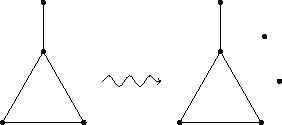
\includegraphics{./img/NPClass/CLIHCLI1.pdf}
        \caption{Supponiamo che $k=3$ e $n=4$. Aggiungiamo $2k-n = 2$ nodi indipendenti. Questi non
        andranno ad influenzare l'esistenza di cricche in $G'$.}
    \end{center}
\end{figure}

Per il caso in cui $k < m$ dobbiamo fare una cosa complementare al caso precedente, dove
aggiungievamo dei nodi per aumentare la dimensione del grafo per raggiungere una dimensione doppia
rispetto a $k$. In questo caso vogliamo ``aumentare $k$ in $G'$'', ovvero aumentare il numero di
nodi in $G$ di un fattore $p$, in modo che $(m+p)$ sia uguale a $2(k+p)$. In questo modo $k + p$
rappresenterebbe il ``$k$ aumentato'' in $G'$, e con $k+p = (m+p)/2 = n'/2$ potremmo dare in input
$G'$ all'algoritmo per $\HALFCLIQUE$. I nuovi $p$ nodi devono essere collegati opportunamente, in
modo che l'esistenza di una cricca di dimensione $k+p$ in $G'$ corrisponda all'esistenza di una
cricca di dimensione $k$ in $G$. Per garantire ciò questi nodi vengono collegati a tutti i nodi di
$G$ e ai nuovi nodi aggiunti. In questo modo non influiscono sull'esistenza di cricche in $G$.

Quanti nodi dobbiamo aggiungere a $G$? Cerchiamo un valore $p$ tale che la dimensione di $G'$, data
da $m + p$, coincida con $2(k + p)$. Di conseguenza doppiamo aggiungere un numero di nodi uguale a
$m - 2k$, connessi a tutti gli altri nodi del grafo. I nodi aggiunti fanno sicuramente parte di una
qualsiasi cricca di $G$. Inoltre se $G'$ ha una cricca di dimensione $k+p$ togliendo i nodi aggiunti
otteniamo una cricca di dimensione $k$.

\begin{figure}[h]
    \begin{center}
        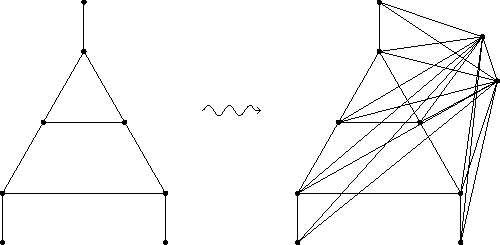
\includegraphics{./img/NPClass/CLIHCLI2.pdf}
        \caption{Supponiamo che $k=3$ e $n=8$. Aggiungiamo $n-2k = 2$ nodi che formano una cricca e
            li colleghiamo agli altri nodi di $G$}
    \end{center}
\end{figure}

Con questo esempio abbiamo modo di vedere una proprietà generale dei problemi $\NPClass$-completi:
per i problemi $\NPClass$-completi esistono in genere dei casi particolari patologici che catturano
l'essenza del problema sua versione generale.

\subsection{$\LIP$ è $\NPClass$-completo}

Consideriamo un'altra classe di problemi importanti $\NPClass$-completi: i problemi di
programmazione intera. Abbiamo un sistema di disequazioni lineari, con variabili
$x_{1},\dotsc,x_{n}$, e ci chiediamo se questo sistema ha una soluzione intera. Il vincolo di
interezza complica il problema, poichè sappiamo che la versione di questo problema che ammette
soluzioni in $\Real$ ha come algoritmo risolutivo l'algoritmo del simplesso, di complessità cubica
(e quindi $\LP \in \PClass$) . $\LIP$ (Linear Integer Programming) è in in $\NPClass$, poichè la
verifica di una soluzione è banale.

Cosa possiamo ridurre a $\LIP$ per dimostrare la sua completezza? In principio possiamo ridurre
tutto, dato che la programmazione lineare intera è molto flessibile e permette di modellare molti
problemi. Vediamo una riduzione da $\SAT$.

Supponiamo, per esempio, di avere tre clausole: $\set{A,\lnot B},\set{A,\lnot C},\set{\lnot A,B}$.
Come variabili per $\LIP$ prendiamo le variabili proposizionali. Dopodiché dobbiamo limitare il
range di queste due variabili a 0 e 1: $A \geq 0$, $A \leq 1$, $B \geq 0$, $B \leq 1$, e così via.
A questo punto dobbiamo imporre che le clausole siano soddisfatte. Di conseguenza vogliamo che i
valori numerici associati alle clausole siano $\geq 1$. Ogni clausola può essere espressa come
somma dei valori dei letterali. Per esprimere la negazione di un letterale $B$ usiamo $1 - B$.
Questo procedimento, che può essere generalizzato a formule arbitrarie in CNF, è illustrato in
Figura \ref{img:SATLIP}.

\begin{figure}[h]
    \begin{center}
        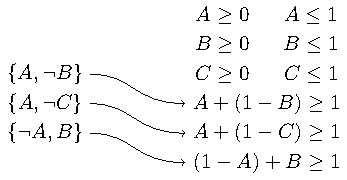
\includegraphics{./img/NPClass/SATLIP.pdf}
        \caption{Esprimiamo i vincoli di $\SAT$ mediante semplici disequazioni.}
        \label{img:SATLIP}
    \end{center}
\end{figure}

\subsection{$\HAMPATH \leq \LIP$}

Per dare un'idea della flessibilità di $\LIP$ nel modellare i problemi vediamo una riduzione da
$\HAMPATH$ a $\LIP$.

Definiamo delle variabili $X_{n,u}$, che esprimono il fatto che il nodo $n$-esimo del cammino
hamiltoniano sia $u$. Vogliamo imporre che i nodi del cammino siano adiacenti in $G$. Esprimiamo
ciò con il seguente vincolo lineare:
\begin{equation*}
    \forall u,v.(u,v) \notin E. X_{i,u} + X_{i+1,v} \leq 1
\end{equation*}
che significa, letteralmente, se due nodi $u$ e $v$ non sono adiacenti in $G$, se al passo $i$
scelgo $u$ al passo $i+1$ non scelgo $v$, e, viceversa, se al passo $i+1$ scelgo $v$ al passo $i$
non scelgo $u$. Ovviamente è lecito che ai passi $i$ e $i+1$ non scelga nessuno dei due.

Vogliamo inoltre che ogni nodo sia toccato una sola volta. Esprimiamo questa condizione con il
seguente vincolo:
\begin{equation*}
    \forall i,n \sum_{i}X_{i,n} = 1
\end{equation*}

Queste due equazioni di vincolo sono sufficienti (insieme alle soliti vincoli di range sulle
variabili a $\set{0,1}$) a modellare $\HAMPATH$.
